\documentclass{ExcelAtFIT}
%\documentclass[czech]{ExcelAtFIT} % when writing in CZECH
\documentclass[slovak]{ExcelAtFIT} % when writing in SLOVAK


%--------------------------------------------------------
%--------------------------------------------------------
%	REVIEW vs. FINAL VERSION
%--------------------------------------------------------

%   LEAVE this line commented out for the REVIEW VERSIONS
%   UNCOMMENT this line to get the FINAL VERSION
%\ExcelFinalCopy


%--------------------------------------------------------
%--------------------------------------------------------
%	PDF CUSTOMIZATION
%--------------------------------------------------------

\hypersetup{
	pdftitle={Chatbot pro Smart City},
	pdfauthor={Bc. Ján Jusko},
	pdfkeywords={chatbot, konverzačný agent, užívateľské rozhranie}
}

\lstset{ 
	backgroundcolor=\color{white},   % choose the background color; you must add \usepackage{color} or \usepackage{xcolor}; should come as last argument
	basicstyle=\footnotesize\tt,        % the size of the fonts that are used for the code
}

%--------------------------------------------------------
%--------------------------------------------------------
%	ARTICLE INFORMATION
%--------------------------------------------------------

\ExcelYear{2018}

\PaperTitle{Chatbot pro Smart City}

\Authors{Ján Jusko*}
\affiliation{*%
  \href{mailto:xjusko00@stud.fit.vutbr.cz}{xjusko00@stud.fit.vutbr.cz},
  \textit{Faculty of Information Technology, Brno University of Technology}}
%%%%--------------------------------------------------------
%%%% in case there are multiple authors, use the following fragment instead
%%%%--------------------------------------------------------
%\Authors{Jindřich Novák*, Janča Dvořáková**}
%\affiliation{*%
%  \href{mailto:xnovak00@stud.fit.vutbr.cz}{xnovak00@stud.fit.vutbr.cz},
%  \textit{Faculty of Information Technology, Brno University of Technology}}
%\affiliation{**%
%  \href{mailto:xdvora00@stud.fit.vutbr.cz}{xdvora00@stud.fit.vutbr.cz},
%  \textit{Faculty of Information Technology, Brno University of Technology}}

\Keywords{chatbot --- konverzačný agent --- užívateľské rozhranie}

\Supplementary{\href{https://www.kroko.live}{Informačná webová stránka}, \href{https://www.facebook.com/messages/t/BrnenskyBot}{Messenger bot}}

%--------------------------------------------------------
%--------------------------------------------------------
%	ABSTRACT and TEASER
%--------------------------------------------------------


\Abstract{
Táto práca popisuje vývoj chatbota pre štatutárne mesto Brno. Chatbot je moderý komunikačný prostriedok založený na konverzácii človeka s počítačom prirodzeným spôsobom prostredníctvom textovej interakcie. Motiváciou je skutočnosť, že spôsob komunikácie samosprávnej časti so svojimi obyvateľmi sa stáva zastaralým. Obyvateľom miest zvyčajne nie je poskytnutý jeden, unifikovaný zdroj informácií a noviniek ale viacero. Práve preto je pre mnohých obyvateľov náročné získavať aktuálne informácie o dianí v samospráve. Tento problém sa snažíme vyriešiť vytvorením konverzačného agenta --- chatbota, s ktorým obyvatelia samosprávy môžu komunikovať prirodzeným jazykom a jednoduchým spôsobom tak dopytovať a prijímať požadované informácie.
%
Výsledkom práce je kompletný návrh aj implementácia chatovacieho robota, ktorý zvláda ako obecné, tak aj Brnu-špecifické otázky. Hlavným prínosom tejto práce je priblíženie samosprávy k obyvateľstvu a uľahčenie získavania informácií spôsobom primeraným dnešnej modernej dobe.
}

%Backup PZ:
%\Abstract{
%Spôsob komunikácie samosprávnej časti so svojimi obyvateľmi sa stáva zastaralým. Obyvateľom miest zvyčajne nieje poskytnutý jeden, unifikovaný zdroj informácií a noviniek ale viacero. Práve preto je pre veľkú časť obyvateľstva náročné získavať aktuálne informácie o dianí v samospráve. Tento problém sa snažíme vyriešiť vytvorením konverzačného agenta --- chatbota, s ktorým obyvatelia samosprávy môžu komunikovať prirodzeným jazykom a jednoduchým spôsobom tak dopytovať a prijímať požadované informácie.
%
%Táto práca popisuje vývoj chatbota pre štatutárne mesto Brno. Výsledkom je kompletný návrh aj implementácia chatovacieho robota ktorý zvláda ako obecné, tak aj Brnu-špecifické otázky. Hlavným prínosom tejto práce je priblíženie samosprávy k obyvateľstvu a uľahčenie získavania informácií spôsobom primeraným dnešnej modernej dobe.
%}

\Teaser{
	\TeaserImage{diagram2.jpg}
}

%PZ: co takhle vele krokodýlka (ozdoba dobrá, ale nic moc informace) dát nějakou krátkou ukázečku dialogu - ne dlohého, ale třeba vtipného... ???

%PZ:... obrázek te%d suser, nicméně možná by se dal k tomu textu nahoře dát třeba "ksich člověka" - klidně Váš a toho krokodýla dole udělat většího, jako že to řeklo "Brno". Ono to trochu je vidět, ale toto by mělo "bít do očí...

% Dakujem, zapracujem

\begin{document}

\startdocument


%--------------------------------------------------------
%--------------------------------------------------------
%	ARTICLE CONTENTS
%--------------------------------------------------------

%--------------------------------------------------------
%--------------------------------------------------------
%--------------------------------------------------------
%--------------------------------------------------------
\section{Úvod}

Predstava moderného a pokrokového mesta pre mnohých ľudí znamená jednoduchý prístup k informáciám a ich interaktívne podanie. V dnešnej uponáhľanej dobe však obyvatelia miest nemajú čas prehľadávať zastarané weby samospráv a preto sa naskytá otázka ako zefektívniť komunikáciu úradov a magistrátu s obyvateľmi. 

%PZ: "lustrovat" je hodně ostré, "zastaralé" se vyskytuje v tomto a hned v dalším odstavci, zvažte změnu.

Spôsob komunikácie samosprávnych častí so svojimi obyvateľmi sa stáva zastaralým. Obyvateľom miest zvyčajne nie je poskytnutý jeden, unifikovaný zdroj informácií a noviniek, ale viacero. Práve preto je pre veľkú časť obyvateľstva náročné získavať aktuálne informácie o dianí v samospráve. Naskytá sa dopyt po jednom, unifikovanom a zároveň modernom zdroji informácií ktorý si ľudia rýchlo osvoja a stane sa ich prvým bodom kontaktu so samosprávou. 

Aktuálny stav komunikácie samosprávy s obyvateľom predstavujú konvenčné prístupy -- webové stránky, vývesné tabule, rozhlasové hlásenia, atď. Medzi silné stránky patrí hlavne ich zaužívanosť medzi ľuďmi ale aj jednoduchosť na implementáciu a správu aj malými obcami. K nedostatkom určite patrí nesúrodosť, komplikovaná dostupnosť a neaktuálnosť.

Náš návrh spočíva v spojení všetkých relevantných dát do jedného kanála ktorý je schopný na vyžiadanie ihneď odpovedať a podať informácie občanom. Ako veľkú výhodu vidíme v jednoduchosti osvojenia si a použitia nami navrhovaného kanála. Navrhované riešenie totiž dokáže spracovávať dotazy v prirodzenom jazyku človeka a rovnako aj odpovedá v prirodzenom jazyku. Dotazy je možné podávať prostredníctvom dvoch textových chatovacích kanálov --- Facebook Messenger a webový chat na stránke projektu.

%PZ: ylo by dobré napsat, že to je textovou konverzací - je to asi "jasné", ale někde by to mělo být explicitně. Myslím také, že by se screenshot nebo tak něco, hodilo do úvodního obrázku k nadpisu práce.

Naše navrhované riešenie -- mestský chatbot Kroko má za cieľ modernizovať spôsob komunikácie samosprávy s obyvateľmi a priblížiť sa im. Opýtať sa chatbota na Facebooku ``Do kdy musím zaplatit daň za mého psa?'' a okamžite dostať odpoveď znie určite veľmi lákavo pre väčšinu ľudí.


\section{Východiská}

%PZ: co třeba jen "Výhodiska", ono v tom moc teorie není...

\subsection{Konverzačné užívateľské rozhranie}
Ešte pred pár rokmi sa počítače ovládali výhradne pomocou myši a klávesnice. Dnes, s nástupom nových technológií, virtuálnej reality a umelej inteligencie potrebujeme oveľa sofistikovanejšie spôsoby.

Konverzačné užívateľské rozhranie (ďalej len CUI - Conversational User Interface) je obecne rozhranie, ktoré napodobňuje konverzáciu so skutočným človekom prostredníctvom prirodzeného jazyka. \cite{brownlee_2018} Namiesto komunikácie s počítačom vo forme technických skratiek, akcií a syntakticky špecifických príkazov, komunikuje užívateľ svojím prirodzeným jazykom a počítaču jednoducho hovorí resp. napíše, čo má robiť.

Idea počítačového systému ovládaného konverzovaním nie je novinka. Ako prvý ju využívali, síce iba v rovine science-fiction, tvorcovia literatúry a kinematografie. K vývoju reálnych systémov s CUI však dochádza až v nedávnej dobe, teda začiatkom druhej dekády 21. storočia. \cite{mielke_2016} Dôvodom toho je, že technológie potrebné k implementácii takéhoto rozhrania konečne dospeli do stavu, kedy je praktické ich použiť. Dvojica veľmi úzko prepojených odvetví informačných technológií, ktorá stojí za pokrokom CUI je odbor spracovania prirodzeného jazyka (NLP - Natural Language Processing) a umelá inteligencia (AI - Artificial Intelligence).

\subsection{Konverzačný agent --- chatbot}
Konverzačný agent (CA --- Conversational Agent) je systém s konverzačným
užívateľským rozhraním. Takýto agent predstavuje praktickú implementáciu CUI spojeného s NLP a ďalšími komponentami ako NLU (Natural Language Understanding), Speech to Text Recognition alebo znalostnou databázou.

Jednou z charakteristík kvality CA je jeho schopnosť zmysluplných výmien strán dialógu. Výmenu definuje literatúra analogicky k výmene v hre -- \textit{\uv{turn}}. 
Účastníci konverzácie sa striedajú v rozprávaní (output) a počúvaní (input). \cite{jurafsky_2019} Jedna výmena môže pozostávať i z jediného slova ale i niekoľkých viet. Najjednoduchšie systémy zvládajú jedinú výmenu, tie sú obecne jednoduché question-answering (FAQ) alebo command-and-control systémy.

Zložitejšie systémy, ktoré zvládajú odpovedať na základe istých ``zapamätaných`` informácií a držať tak zmysluplnú konverzáciu viac ako jeden \textit{turn} musia implementovať podporné mechanizmy.
Je nutné ukladať aktuálny kontext konverzácie s užívateľom ale tiež aj jeho priebežne zdieľané informácie ako vek, pohlavie, záujmy, obľuby, atď.


\section{Metodológia}

Táto kapitola slúži ako rozšírené zadanie. Obsahuje návrh konceptu chatbota --- čo by mal zvládať, ako by sa mal prezentovať, čomu sa má vyvarovať, \dots

\subsection{Vedomostná doména}
Mesto Brno má veľkú snahu prezentovať sa ako moderné miesto pre život. Preto chce svojím obyvateľom poskytnúť nový, inovatívny komunikačný kanál ktorý je možné využiť k získaniu informácií o meste.

Vedomostná doména chatbota predstavuje množinu vedomostí, ktoré dokáže poskytnúť --- veci, ktoré \emph{``umí``}. Vytvorenie návrhu vedomostnej domény vychádza zo skúseností zamestnancov, ktorí analyzovali aké otázky ľudia pokladajú najčastejšie.

\vspace{2mm}
\textit{Kontakty na zamestnancov mesta}

%PZ: formátově to není ideáoní, zkuste třeba ne jako subsection, ale jinak, možná kurzívou???

\noindent Podľa vyjadrenia viacerých zamestnancov magistrátu mesta Brno, vyhľadávanie kontaktu na zamestnancov mesta, úradníkov a politikov je najčastejší dôvod prečo ľudia navštevujú web \url{www.brno.cz}.

Navrhovaný chatbot bude schopný rozoznať zámer užívateľa vyhľadať kontakt (telefón, e-mail, adresu pracoviska) na konkrétnu osobu podľa mena (Ján Novák) alebo pozície (primátor mesta).

\vspace{2mm}
\textit{Potrebujem si vybaviť}

\noindent Veľmi častou sekciou oficiálneho webu mesta je aj \emph{Potřebuji si vyřídit}. Obsahuje súrhnné informácie k najčastejším úkonom v správe mesta ako napríklad vybavenie cestovného dokladu, občianského preukazu, registrácie vozidla alebo oprávnenia k rezidentnému parkovaniu. Informácie z nej sme zaradili i do vedomostnej domény nášho konverzačného agenta.

%PZ: možná není šikovné mít use cases jen podle toho, kdo co často potřeabuje. Ne, že by to bylo nemožné, ale je to takpvé "oportunistické". Navrhuji možná vynechat to "Druhou nejnavštěvovanější", ale dát třeba "Velmi častou"...

\newpage
\textit{Multimodálna navigácia mestom}

\noindent S možnosťou získať užívateľovu aktuálnu polohu z aplikácie Messenger, je konverzačný agent vhodným ``médiom`` pre navigáciu mestom. Medzi podporované spôsoby dopravy po meste zahrňujeme celú sieť mestskej hromadnej dopravy a pešie presuny. Naším cieľom je vytvoriť užívateľsky prívetivejšie riešenie ako aktuálne najpoužívanejší vyhľadávač spojení IDOS\footnote{IDOS -- \url{https://jizdnirady.idnes.cz/brno/spojeni/}}.

\subsection{Branding}
Persona chatbota je spojená s ``najznámejším Brnenským zvieraťom`` --- Brnenský drak visiaci v budove starej radnici. Chatbot bude vystupovať pod menom \textbf{Kroko} a logom (vid. obrázok \ref{kroko}). Bude komunikovať v milom a slušnom tóne.

\begin{figure}[h]
	\centering
	
\includegraphics[width=0.5\linewidth]{resized2.png}
	\caption{Logo, pod ktorým bude vystupovať chatbot Kroko.}
	\label{kroko}
\end{figure}


\section{Implementácia}
Táto kapitola sumarizuje ako základné prvky technickej stránky chatbota, tak aj zaujímavé riešenia niektorých problémov.

\subsection{Technická architektúra}
Aplikácia chatbota Kroka je navrhnutá a vytvorená ako webová služba dostupná prostredníctvom HTTP protokolu. Rozhranie aplikácie je definované podľa pravidiel REST API architektúry. Chatbot prijíma HTTP requesty obsahujúce identifikátor užívateľa a jeho správu. Následne odpovedá s HTTP response obsahujúcou jeho odpoveď.

Back-end aplikácie je zodpovedný za udržiavanie kontextu dialógu, analýzu vstupných správ, určenie zámeru užívateľa a nakoniec vytvorenie vhodnej odpovedi k vráteniu.
Samotná aplikácia využíva dve služby tretích strán --- parser českého jazyka \emph{UDPipe} a komponentu na určovanie zámeru užívateľa \emph{Wit.ai}.

\newpage
\textit{UDPipe}

\noindent UDPipe\footnote{UDPipe -- \url{http://lindat.mff.cuni.cz/services/udpipe/}} je nástroj schopný rozparsovať vetu a vytvoriť jej syntaktickú analýzu. Dôležité je zdôrazniť, že pracuje s českou gramatikou čo je nutné k chatbotovi Krokovi. Okrem iného, dokáže aj určovať slovné druhy vo vete a základnú formu slov, tzv. \emph{stemming}.

\begin{figure}[h]
	\centering
	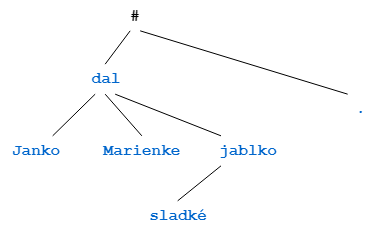
\includegraphics[width=1\linewidth]{DependencyTree.png}
	\caption{Syntaktická analýza --- strom závislostí.}
	\label{tree}
\end{figure}

\vspace{5mm}
\textit{Wit.ai}

\noindent Nástroj Wit.ai poskytuje spoločnosť Facebook ako trénovateľnú umelú inteligenciu schopnú detekovať zámer (\emph{intent}) zo vstupného textu.

\begin{figure}[h]
	\centering
	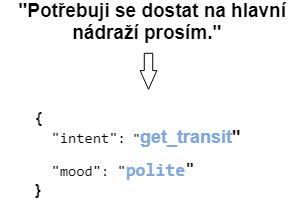
\includegraphics[width=0.65\linewidth]{witai.png}
	\caption{Príklad využitia nástroja wit.ai.}
	\label{wit}
\end{figure}


\subsection{Frame-based architektúra}

Chatbot Kroko využíva pri riadení jednotlivých use-casov tzv. \emph{frame-based} architektúru.
S \emph{frame-based} architektúrou, informácie nutné k extrahovaniu z užívateľových dotazov sú reprezentované ako množina rámcov (frames), každý obsahujúci jeden alebo viac slotov ktoré zároveň nesú informáciu o tom, aké typ hodnôt môžu nadobúdať. \cite{jurafsky_2019}
Tento prístup bol predstavený v roku 1977 implementovaný do cestovného asistenta GUS schopného vyhľadávať a rezervovať letenky. Pre zámer vyhľadávania letenky je rámec slotov znázornený na obrázku \ref{alto}.

\begin{figure}[h]
  \centering
  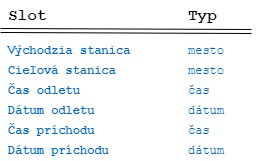
\includegraphics[width=0.7\linewidth]{Slots.jpg}
  \caption{Rámce a sloty pre use-case cestovného agenta.}
  \label{alto}
\end{figure}

\noindent Interakcia s takýmto agentom prebieha pokiaľ sa príslušnými hodnotami nenaplnia všetky sloty. 
Samotné typy môžu byť ďalej hierarchicky delené a získavané od užívateľa v samostatnom rámci. Napríklad dátum človek nemusí špecifikovať vždy naraz celý, preto sa chatbot môže dopytovať na ostatné zložky dátumu (deň, mesiac, rok).

\subsection{Udržiavanie kontextu}

Pre kvalitný užívateľský zážitok je nutné v konverzácii udržiavať kontext. Kontext sa zvyčajne nastavuje pri odoslaní odpovede užívateľovi. Následne pri prijatí ďalšej správy od užívateľa dokážeme určiť, čoho sa odpoveď týka, resp. v akom kontexte užívateľ hovorí.

Mechanizmy, ako najlepšie udržiavať kontext u konverzačných agentov a chatbotov zatiaľ nie sú v literatúre popísané a preto sme museli navrhnúť vlastný systém. Kontext konverzácie s užívateľom je v našom chatbote reprezentovaný perzistentným databázovým objektom ktorý sa skladá z nasledovných dát.

\begin{itemize}
    \item \textbf{user\_id} -- jedinečný identifikátor užívateľa
    \item \textbf{context\_keyword} -- určuje v akom use-case sa pohybujeme
    \item \textbf{context\_value} -- určuje, čo posledné chatbot odpovedal
    \item \textbf{context\_additional\_info} -- pomocné dáta slúžiace ku krátkodobému uloženiu
\end{itemize}

Dobrým príkladom, kedy využívame ukladanie kontextu je dopytovanie doplňujúcich informácií, ktoré potrebujeme zistiť od užívateľa k dokončeniu istého use-case.
Na obrázku \ref{kontext} je znázornené nastavenie kontextu. Následne pri prijatí odpovede už chatbot vie, že adresa \emph{Božetěchova 2} predstavuje východzie miesto multimodálnej navigácie, ktorú chce užívateľ použiť.

\begin{figure}[h]
  \centering
  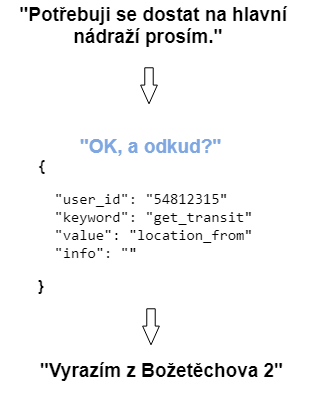
\includegraphics[width=0.7\linewidth]{context.png}
  \caption{Riadenie kontextu.}
  \label{kontext}
\end{figure}

\section{Testovanie}
Po implementácii chatbota bude nasledovať užívateľské testovanie. V príprave sú podrobné end-user testy ktoré budú merať viacero faktorov. Užívatelia budú hodnotiť kvalitatívne črty --- jednoduchosť použitia, intuitívnosť, zážitok \ldots.

Pri porovnaní s tradičnými informačnými kanálmi budeme merať časový rozdiel v nájdení rovnakej informácie prostredníctvom chatbota vs. prostredníctvom pôvodných kanálov.

\section{Záver}

Práca sa zaoberá vytvorením nového, moderného spôsobu komunikácie a predávania informácií medzi samosprávou a obyvateľmi. Navrhovaným riešením je textový chatbot Kroko dostupný rozšírenej platforme Facebook Messenger.

Práca je tvorená v spolupráci so štatutárnym mestom Brno. Spolupráca spočívala najmä vo vytvorení ucelenej predstavy o cieľovej skupine používateľov a potenciálne najčastejších prípadoch užitia.
Zo spolupráce vyplynuli 3 hlavné scenáre, ktorým bude chatbot schopný porozumieť a podať príslušné informácie. \\
Jedná sa o navigáciu mestom kombináciou viacerých dopravných možností, poskytnutie kontaktu na mestských zamestnancov a poskytnutie informácií o najčastejších úkonoch v správe mesta (vybavenie cestovného dokladu, vodičského oprávnenia, rezidentného parkovania, \dots).

Pokračovaním tejto práce bude diplomový projekt. V ňom bude podrobne popísaná implementácia chatbota spolu s vyhodnotením užívateľského testovania, jeho funkčných vlastností a miery využitia obyvateľstvom.

%--------------------------------------------------------
%--------------------------------------------------------
%--------------------------------------------------------
%	REFERENCE LIST
%--------------------------------------------------------
%--------------------------------------------------------
\phantomsection
\bibliographystyle{unsrt}
\bibliography{2019-ExcelFIT-ShortName-bib}

%--------------------------------------------------------
%--------------------------------------------------------
%--------------------------------------------------------
\end{document}